\documentclass{article}
%%%%%%%%%%%%%%%%%%%%%%%%%%%%%%%%%%%%%%%%%%%%%%%%%%%%%%%%%%%%%%%%%%%%%%%%%%%%%%%
% PREAMBLE
%%%%%%%%%%%%%%%%%%%%%%%%%%%%%%%%%%%%%%%%%%%%%%%%%%%%%%%%%%%%%%%%%%%%%%%%%%%%%%%
\usepackage{mathtools}
\usepackage{algorithm}
\usepackage{algorithmic}
\usepackage{fancyvrb}
\usepackage{booktabs}
\usepackage{rotating}
\usepackage{listings}
\usepackage{tikz}
\usepackage{float}
\usepackage{hyperref}
\usepackage{subcaption}
\usetikzlibrary{arrows,decorations.pathmorphing,backgrounds,positioning,fit,matrix}
\newcommand{\DepProps}{\textsc{DepProps}}
\usepackage{titling}
\newcommand{\subtitle}[1]{%
  \posttitle{%
    \par\end{center}
    \begin{center}\large#1\end{center}
    \vskip0.5em}%
}
\begin{document}
% TITLE
\title{DM819 - Computational Geometry}
\subtitle{Fall 2015\\Project 2}
% AUTHER
\author{Mikkel Levisen and Jesper Lund}
%DATE
\maketitle
% no page number on first page
\thispagestyle{empty}
\newpage
% TABLE OF CONTENTS
\tableofcontents
% no page number on table of contents page
\thispagestyle{empty}
\newpage
% restart page number counter
\pagenumbering{arabic} 
%%%%%%%%%%%%%%%%%%%%%%%%%%%%%%%%%%%%%%%%%%%%%%%%%%%%%%%%%%%%%%%%%%%%%%%%%%%%%%%
% DOCUMENT START
%%%%%%%%%%%%%%%%%%%%%%%%%%%%%%%%%%%%%%%%%%%%%%%%%%%%%%%%%%%%%%%%%%%%%%%%%%%%%%%
\section{Introduction}
  This report details the implementation of KD-Tree and Range-Tree for 
  $d$-dimensional input. Each tree is constructed from a list of unsorted points
  and is capable of performing orthogonal range queries.
  \subsection{Definitions}
  \begin{itemize}
  	\item a $d$-dimensional point, $p$, consists of real numbers $(p_1,p_2,\dots,p_d)$
  	\item a $d$-dimensional range, $R$, is a hyper-volume defined by $[r_1:r_1']
  	\times[r_2:r_2']\times \dots \times [r_d:r_d']$, where each $r$ is a real number
  \end{itemize}

  \subsection{Range Queries}
  Given a set of points, $P$, and a range object, $R$, a range query consist of
  reporting all points in $P$ which intersect $R$ e.g. a 1-dimensional point
  set $\{1,2,3,4,5\}$ and a range object $[2:4]$ yields $\{2,3,4\}$. 
  
  
  
  %that intersects 
  %a 
  %A point $p \in P$ exists in the range $R$ iff.
  %\[
  %  \forall p_i \in p: \{ R_{i,1}\leq   p_i \leq R_{i,2}\}|\forall i \in \{1,...,n\}, n = dimensions 
  %\]
  %
  %A range query consists of reporting all points, $p$, which lie within a given 
  %range, $R$.
  %An $n$-dimensional point, $P_n$, consist of real numbers 
  %$\{p_1,p_2,\dots,p_n\}$, and an $n$-dimensional range $R_n$ consist of 
  %$[x:x']\times[y:y'] \times \dots \times[z:z']$. A range query consist of 
  %reporting all points $P_n$ in a range $R_n$.
\section{KD-Tree}
This solutions uses elements containing arrays of $d$ floats, each index in the array corresponds to each dimension in the tree.
The solution is a generalized version of the one IN THE BOOK page. 99, where the one in the book uses 2 dimensions, this one instead
generalizes the way it handles each dimension, allowing for an arbitrary number of dimensions.
\subsection{Tree construction - with n-dimensions}
Like in the book, the tree is constructed by splitting the list of points $P$ on it's median based on the current dimension being split.
But unlike the book's version we doesn't just check if depth is even or uneven, we instead formalize the current depth as being
\[
 d = (depth\ mod\ dimension)+1
\]
Where $dimension$ is a constant equal to the number of dimensions.
Note the plus 1 in the implementation, this is because that Lua is 1-indexed, so for a 3-dimensional KD-tree, we need indexes from 1 through 3,
instead of traditional 0 through 2.\\
 \\
To help achieve this, we have a function \texttt{splitListOnMedian}, which uses an selection algorithm to find the median, and then return both the median and set $p_1$,$p_2$.
The points in $p_1$ is all points that are equal or less than the median, the points in $p_2$ is then all points above the median.

The rest of the construction is like like the book's version, call \texttt{BUILDKDTREE} on each set $p_1$,$p_2$ and create a node containing each subtree as it's left and right child, 
and the node will have the value of the median found.\\
 \\
Note: Since the median is inclusive for the left child, we might have unbalanced sets, consider the following set: \{1, 2, 3, 3, 4\}, the median would be 3, but since the behavior for
constructing the children includes the values that are equal to the median in the lesser set, we would have a node with children \{1, 2, 3, 3\} and \{4\}.

\subsection{Searching the tree - with n-dimensions}
Like the algorithm for searching in the book, we have 3 cases.
\begin{itemize}
 \item Current node \texttt{v} we are looking at, is a leaf. This means that we have to check if that node is contained in our range $R$.
 \item Left or right- subtree of \texttt{v} are fully contained, if that's the case, we traverse the tree and report all nodes within.
 \item \texttt{region} are intersecting $R$ but is not fully contained within $R$, this means we have to do the checks again on the children of \texttt{v}.
\end{itemize}
But, unlike the book, we have adapt the algorithm to consider more dimensions, this is done by using the \texttt{region}.
The \texttt{region} is structured just like our $R$, but instead of containing ranges, it contains the minimum and maximum ranges at the current node.

The \texttt{region} starts as a empty set, i.e. we don't know the maximum and minimum at the current nodes. 
But for each subsequent depth in the tree, we update the \texttt{region} like:
\[
    \texttt{region}= 
    \texttt{region} \cup \texttt{region}(child)
\]
Which can be translated to:
\[
    \texttt{region}= 
\begin{cases}
    \texttt{region}_{d,max} = MIN(\texttt{region}_{d,max},halfline),&\text{for left child} \\
    \texttt{region}_{d,min} = MAX(\texttt{region}_{d,min},halfline),& \text{for right child}
\end{cases}
\]
Where halfline, is the value of the median i.e. the value of the current non-leaf node.
This means that we narrows our search by reducing the max-value, and increasing our min-value.\\
 \\
Now checking if the \texttt{region} is fully contained within a range is a simple matter.
The \texttt{region} is fully contained in the ranges when every minimum and maximum foreach dimension of the \texttt{region} is within every range in $R$.\\
 \\
The last step is now if the \texttt{region} is not fully contained, we have to check if it is intersecting with the ranges. This comes down to two cases.
If the \texttt{region} hasn't been constructed yet, so we don't have enoigh information to determine, we have to check further down.
If the \texttt{region} has been constructed, we need to check if any of the ranges of \texttt{region} are within the range $R$ for each dimension respectively, if any of these are true,
the \texttt{region} is intersecting and we need to check the subtrees.\\
Note: The search also uses the same technique as the construction, namely the $d = (depth\ mod\ dimension)+1$, when it comes to dimensions.
 \\
The code is included in the appendix, in \textbf{kdtree.lua}.
\section{Range-Tree}
  A Range-tree is a multi-level data structure for time efficient range queries.
  In 2-dimensional the firs-level of the range tree is a binary search tree on 
  the $x$-coordinate. Each node has an associated data structure for all
  points in its canonical set. The associated data structure is a binary 
  search tree on the $y$-coordinate of the points. 
  To report which points are in a given range is a 1-dimensional range search 
  performed for each dimension, that is, first find all leaf nodes which lie 
  within $[x:x']$ in the first level, then determine which of those nodes 
  $y$-coordinate lie within $[y:y']$ on the second level. 
 \section{Test}
    \subsection{Test Generation}
    Supplied with the code is a test generating script which can create tests of
    arbitrary dimension and size. The tests are stored in directories by 
    dimension.
    
    In a tests consisting of $n$ points in $d$ dimensions a $d$-dimensional 
    volume is constructed with a side length $s = \sqrt[d]{n}$. For each such 
    volume is $1000$ ranges generated with a side length of 
    $rs = \sqrt[d]{0.1 \cdot s^d}$ i.e. each range will contain approximately 
    10\% of the $n$ points. 
\begin{figure}[H]
    \centering
    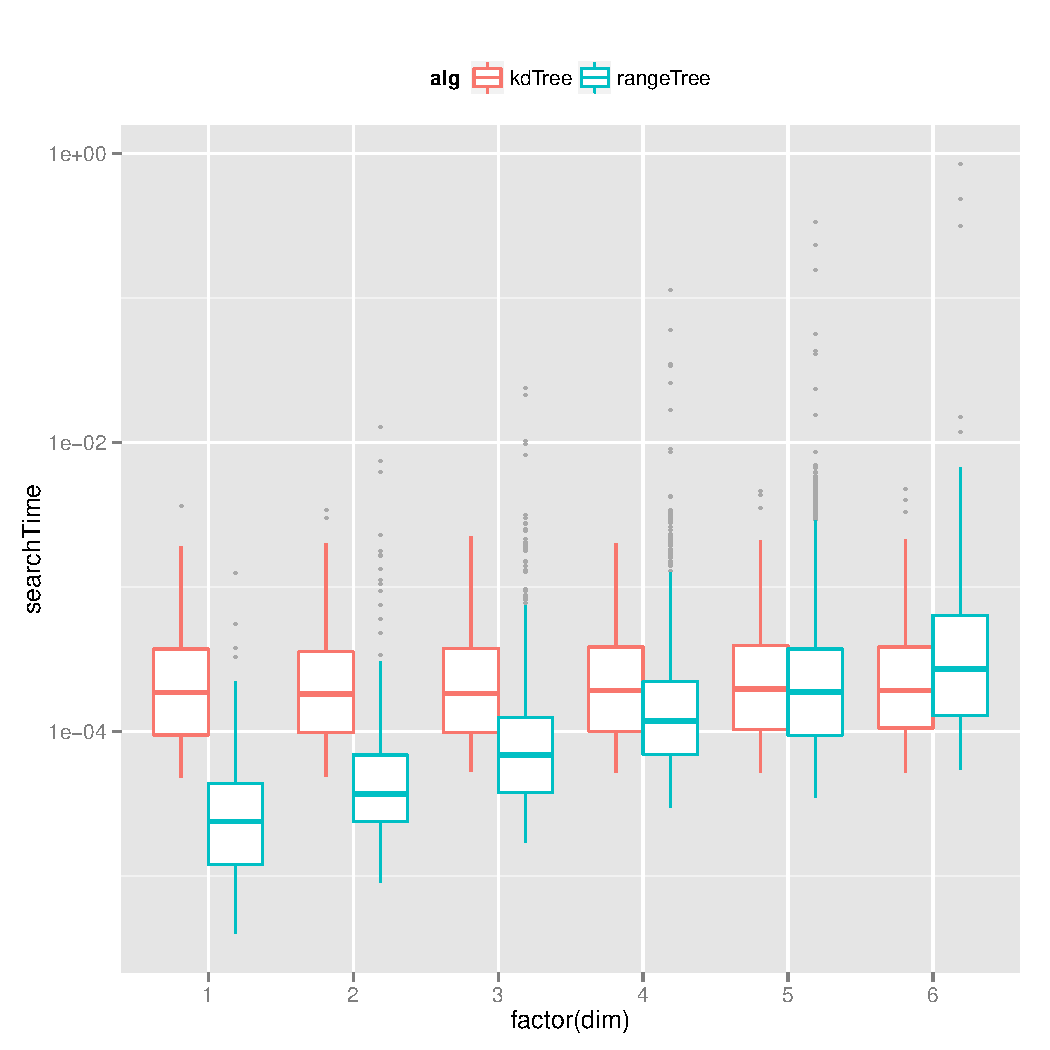
\includegraphics[width=\textwidth]{../src/R/plots/boxplot.pdf}
\end{figure}
\begin{figure}[H]
    \centering
    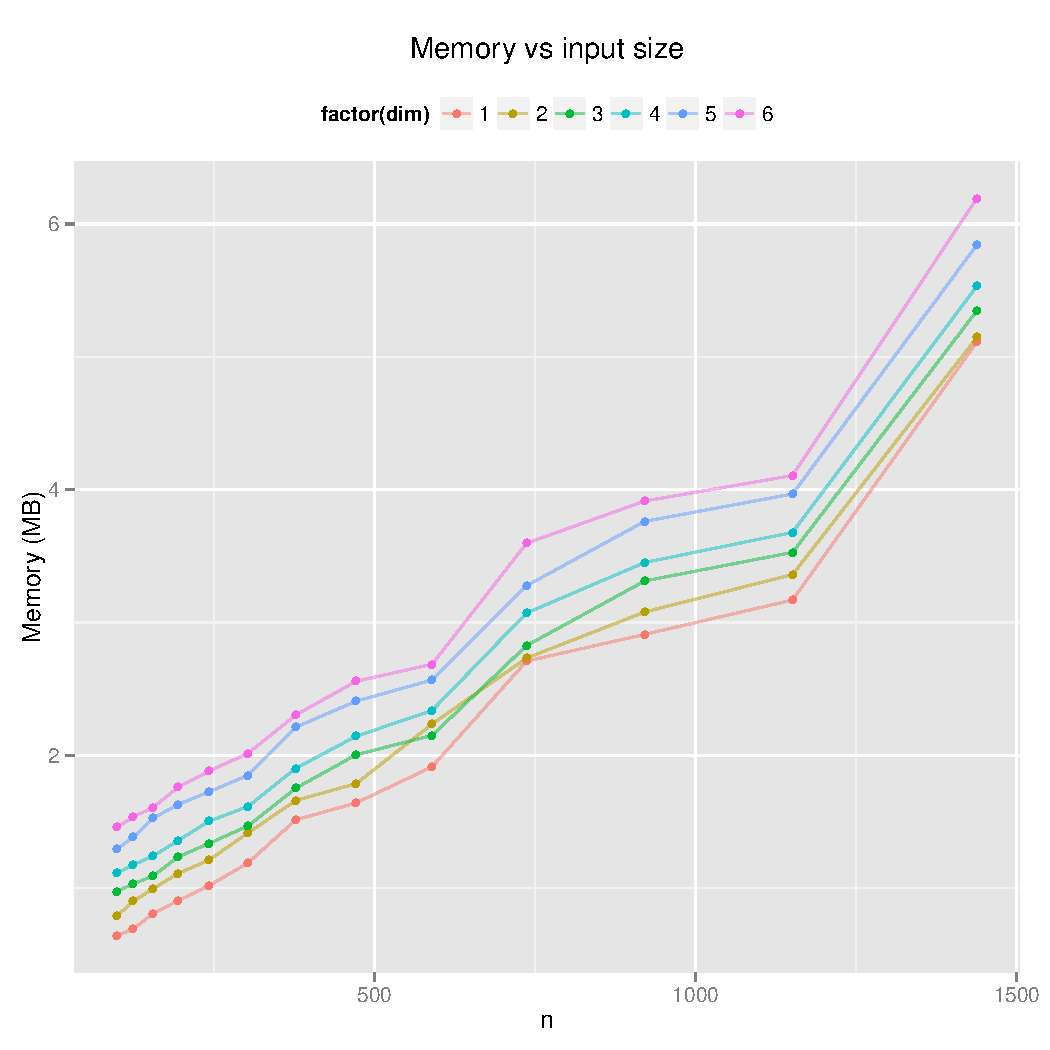
\includegraphics[width=\textwidth]{../src/R/plots/kdmem.pdf}
\end{figure}
\begin{figure}[H]
    \centering
    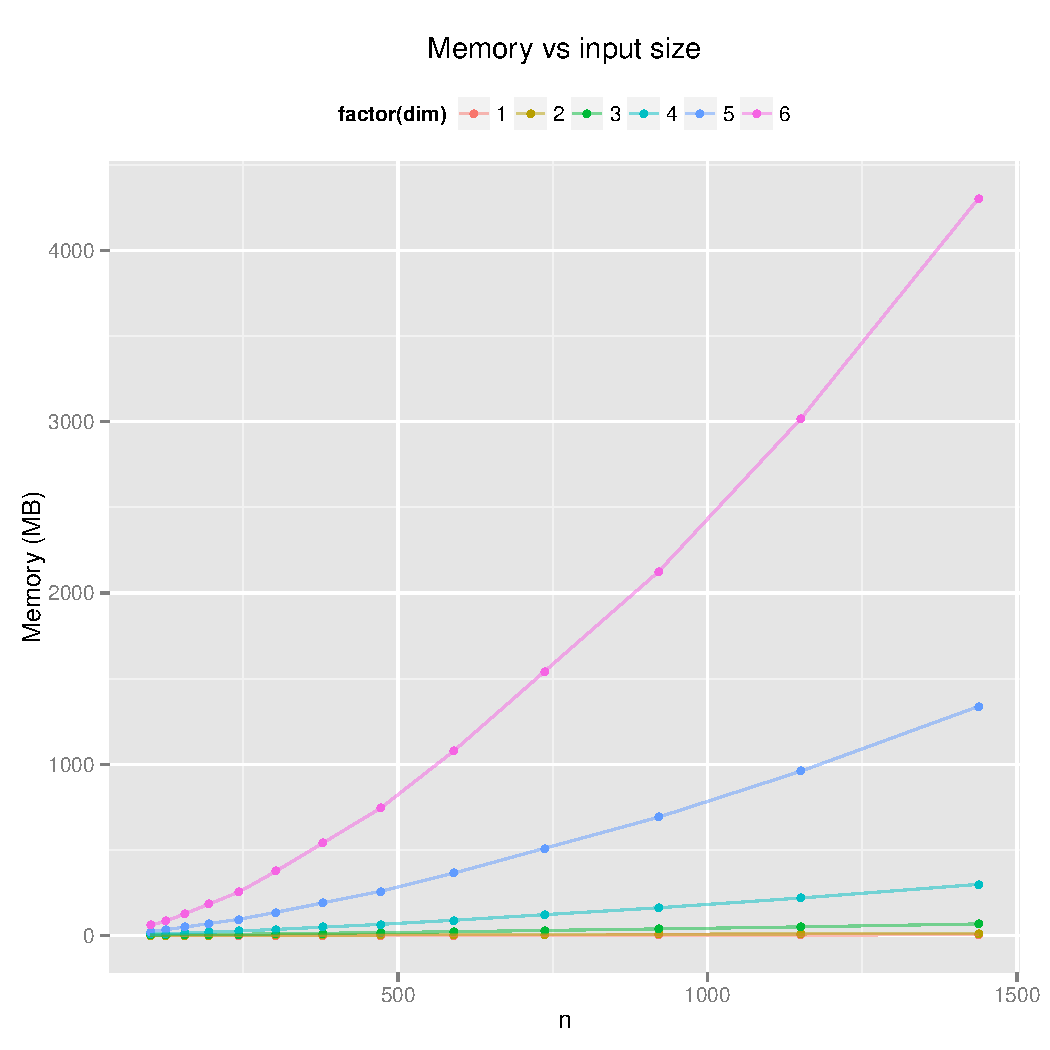
\includegraphics[width=\textwidth]{../src/R/plots/rtmem.pdf}
\end{figure}
\section{Manual}
  \subsection{File Formats}
  \subsubsection{Input}
  The input file format consist of two distinctest parts: \textit{points} and 
  \textit{ranges}. 
  \\
  \\
  Points are real numbers separated by \verb|<TAB>|. 
  \begin{verbatim}
  	<real> \t <real>
  	<real>:<real> \t <real>:<real> [, <integer> \t <integer>]
  \end{verbatim}

  \subsection{Inscrutions}
\subsection{File Structure}
\begin{verbatim}
ROOT
|-- report/
`-- src
    |-- kdtree
    |   |-- inspect.lua
    |   |-- kdtree.lua
    |   `-- test.lua
    |-- R
    |   `-- makePlots.R
    |-- rangeTree
    |   |-- inspect.lua
    |   |-- middleclass
    |   |   `-- middleclass.lua
    |   |-- RangeTree.lua
    |   `-- test.lua
    |-- results/
    |-- runTests.py
    `-- tests
        |-- createCustomTest.lua
        |-- dimension_1/
        |-- dimension_2/
        |-- dimension_3/
        |-- dimension_4/
        |-- dimension_5/
        |-- dimension_6/
        |-- genTestSuite.lua
        `-- inspect.lua
\end{verbatim}

\section{Conclusion}
\end{document}